\begin{figure}
\begin{subfigure}{0.655\textwidth}
\centering
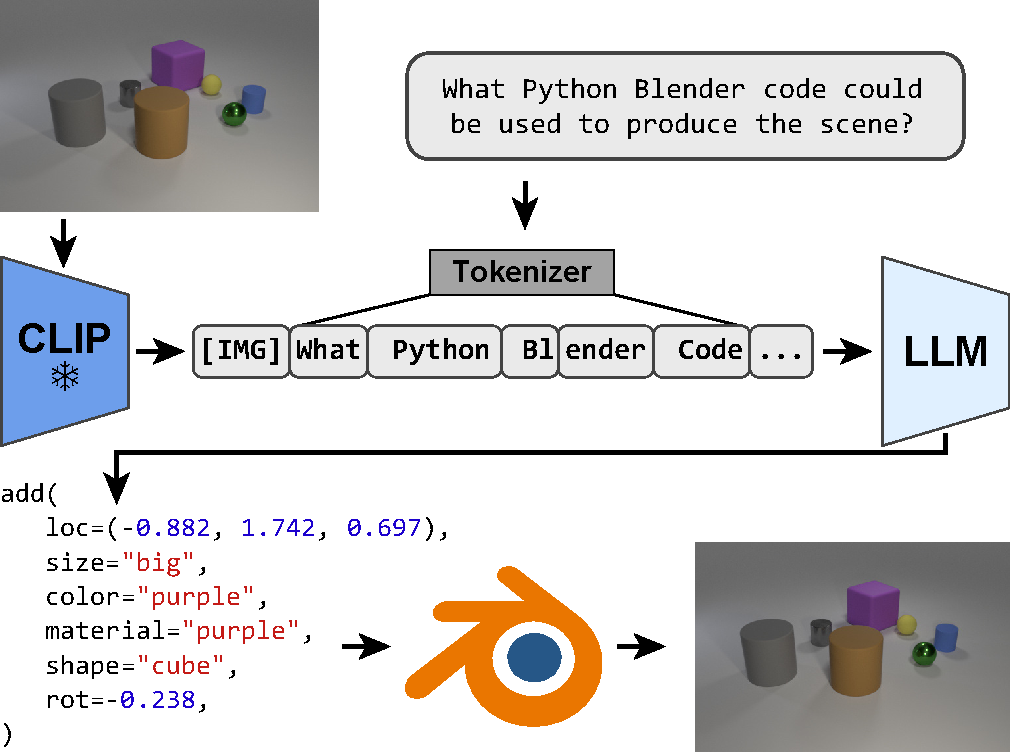
\includegraphics[width=\linewidth]{figures/diagram/pipeline.pdf}
\end{subfigure}
\hfill
\vline
\hfill
\begin{subfigure}{0.325\textwidth}
\centering
\small
\cref{ssec:clevr}: Compositional Generalization\\
\vspace{0.025cm}
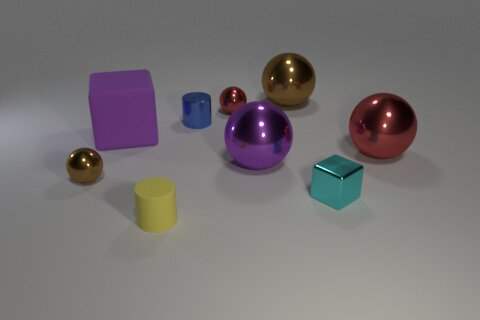
\includegraphics[width=0.400\linewidth]{figures/clevr/input/teaser.jpg}
\hspace{0.025cm}
\raisebox{0.25in}{$\Rightarrow$}
\hspace{0.025cm}
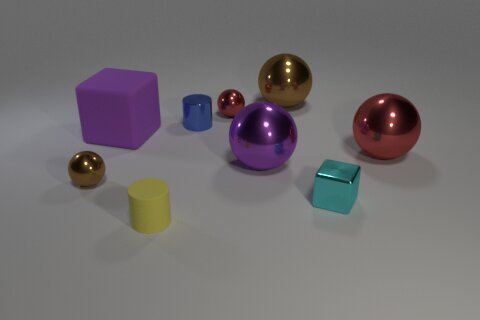
\includegraphics[width=0.400\linewidth]{figures/clevr/output/teaser.jpg}\\
\cref{ssec:parameter_space_generalization}: Parameter-Space Generalization\\
\vspace{0.025cm}

\includegraphics[width=0.400\linewidth]{figures/2d/sparse_checkerboard.pdf}
\hspace{0.025cm}
\raisebox{0.4in}{$\Rightarrow$}
\hspace{0.025cm}
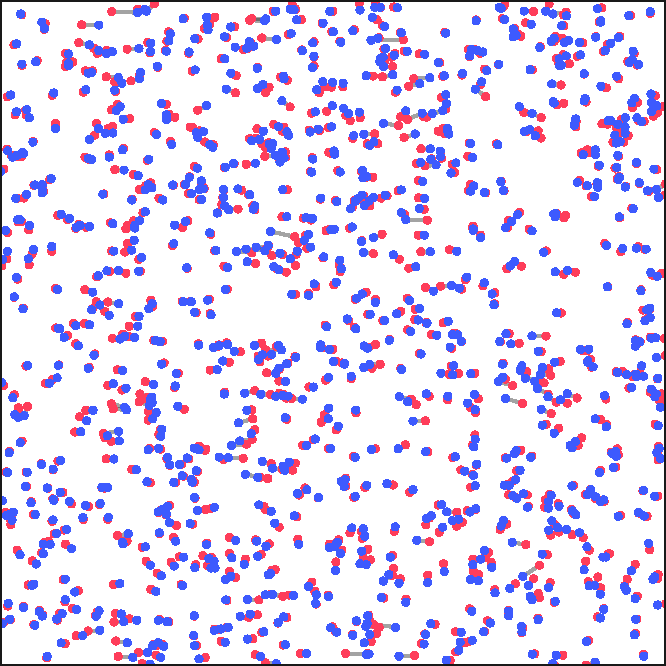
\includegraphics[width=0.400\linewidth]{figures/2d/float_scatter.pdf}\\
\cref{ssec:6dof}: Visual-Domain Generalization\\
\vspace{0.025cm}
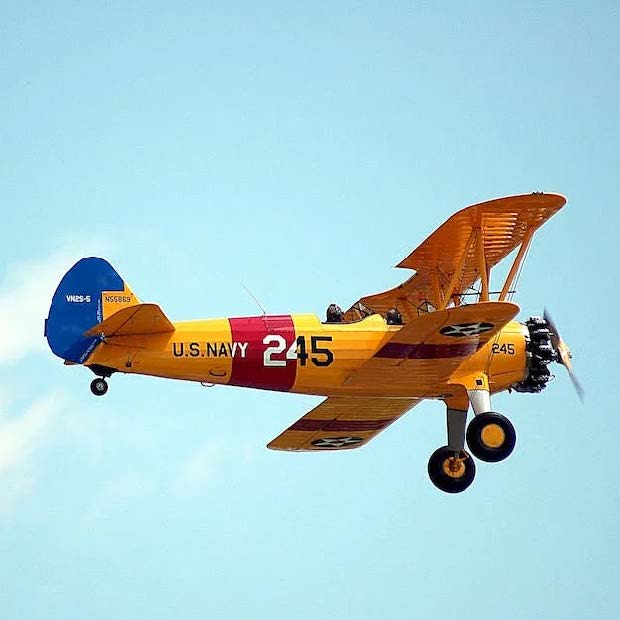
\includegraphics[width=0.400\linewidth]{figures/airplane/6dof/input/teaser.jpg}
\hspace{0.025cm}
\raisebox{0.4in}{$\Rightarrow$}
\hspace{0.025cm}
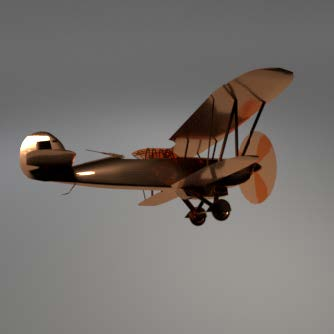
\includegraphics[width=0.400\linewidth]{figures/airplane/6dof/output/teaser.jpg}
\end{subfigure}
\caption{\textbf{IG-LLM.}
We present the Inverse-Graphics Large Language Model (IG-LLM) framework, a general approach to solving inverse-graphics problems.
We instruction-tune an LLM to decode a visual (CLIP) embedding into graphics code that can be used to reproduce the observed scene using a standard graphics engine.
Leveraging the broad reasoning abilities of LLMs, we demonstrate that our framework exhibits natural generalization across a variety of distribution shifts without the use of special inductive biases.
}
\label{fig:teaser}
\vspace{-0.1015cm}
\end{figure}